\documentclass[a4paper,12pt]{report}
\usepackage[T2A]{fontenc}
\usepackage[utf8x]{inputenc}
\usepackage[english, russian]{babel}
\let\myBib\thebibliography
\let\endmyBib\endthebibliography

\renewcommand\thebibliography[1]{\ifx\relax#1\relax\else\myBib{#1}\fi}
\usepackage{amssymb,amsfonts,amsmath,mathtext,cite,enumerate,float}
\usepackage[pdftex]{graphicx} 
\graphicspath{{images/}}

\RequirePackage[labelsep=period]{caption}
\makeatletter
\renewcommand{\@biblabel}[1]{#1.} 
\makeatother

\usepackage{geometry} 
\geometry{left=2cm}
\geometry{right=1.5cm}
\geometry{top=1cm}
\geometry{bottom=2cm} 



%\renewcommand{\thefigure}{\arabic{figure}} 
%\renewcommand{\theequation}{\arabic{equation}} 
\renewcommand{\theenumi}{\arabic{enumi}}
\renewcommand{\labelenumi}{\arabic{enumi}}
\renewcommand{\theenumii}{.\arabic{enumii}}
\renewcommand{\labelenumii}{\arabic{enumi}.\arabic{enumii}.}
\renewcommand{\theenumiii}{.\arabic{enumiii}}
\renewcommand{\labelenumiii}{\arabic{enumi}.\arabic{enumii}.\arabic{enumiii}.}


\bibliographystyle{unsrt}
\begin{document}
Здесь будет титульный лист, присланный из института ближе к сдаче

Использование методов глубокого обучения для предсказания кардиологических временных рядов
\tableofcontents
\chapter{Введение}

Предсказанием и распознаванием болезней человека, его различных характеристик по сигналу ЭКГ занимаются многие группы ученых \cite{about_ekg_sciense1, about_ekg_sciense2}. Медицинские институты собирают данные, ученые исследуют уже известные методы получения и обработки информации о сердечной активности и изобретают новые \cite{get_ekg_signal}. Благодаря развитию медицинских технологий, позволяющих получать ЭКГ сигнал круглосуточно, задачи в этой области становятся все более актуальными. Множество людей сегодня носят фитнес-браслеты, наблюдающие за пульсом человека, создаются модели холтеров, позволяющие получать все более точный сигнал, продаются чехлы для телефонов, способные записывать ЭКГ сигнал в любой удобный момент времени.

Анализируя эту информацию, можно вовремя распознать различные болезни и принять предупредительные меры. Также одной из важных задач анализа ЭКГ сигнала является определение периодов сна/бодрствования человека. Сонливое состояние в течение дня -- одна из главных причин несчастных случаев на дорогах и производстве \cite{accidents}. Как следствие, большой интерес представляет осуществление постоянного контроля за уровнем сонливости лиц, чья работа связана с риском, таких как летчики, водители-дальнобойщики и др.. В настоящее время в промышленности для предотвращения чрезвычайных ситуаций используется наблюдение за поведением людей (открыты ли глаза). 

В данной работе рассказано о способах фильтрации ЭКГ-сигнала, выделении RR-интервалов и методах анализа RR-сигнала. Описаны алгоритмы классификации, показавшие хорошее качество при классификации периодов времени на сон/бодрствование. Также проведены эксперименты по предсказанию заболеваний.
\chapter{Обзор литературы}

\section{Вариабельность сердечного ритма }

Вариабельность сердечного ритма (Heart rate variability, HRV) это явление изменения частоты сердечного ритма.

Вариабельность сердечного ритма сильно зависит от эмоционального \cite{hrv_and_sensitivity, hrv_and_respiratory} и физического \cite{hrv_and_phisical_health} здоровья человека и может использоваться как его показатель.

Существуют два основных причины колебания частоты сердечного ритма \cite{two_rates_hrv}.

\begin{itemize}
	\item Колебания, вызванные дыхательной аритмией. При этом частота сердечных сокращений изменяется в связи с дыханием и можно отследить частоту дыхания.
	\item Низкочастотные колебания артериального давления. Это явление называется волнами Майера \cite{mayer_wave} артериального давления и, как правило, имеют частоты порядка 0,1 Гц.
\end{itemize}

Для наблюдения за сердечным ритмом применяются следующие методы:

\begin{itemize}
	\item ЭКГ (электрокардиография) \cite{EKG};
	\item баллистокардиография  \cite{Ballistocardiograms};
	\item фотоплетизмография \cite{Photoplethysmography}.
\end{itemize}

ЭКГ считается методом, дающим наиболее четкий сигнал.

\subsection{ЭКГ}

Электрокардиограмма – это запись колебаний разности потенциалов, возникающих на поверхности возбудимой ткани или в окружающей сердце проводящей среде при распространении волны возбуждения по сердцу.\cite{ekg1} Запись ЭКГ производится с помощью электрокардиографов и различных систем отведений ЭКГ. Каждое отведение регистрирует разность потенциалов, существующую между двумя определенными точками электрического поля сердца, в которых установлены электроды. Пример ЭКГ можно увидеть на рис. \ref{ris:RR}.

\begin{figure}[h]
	\begin{center}
		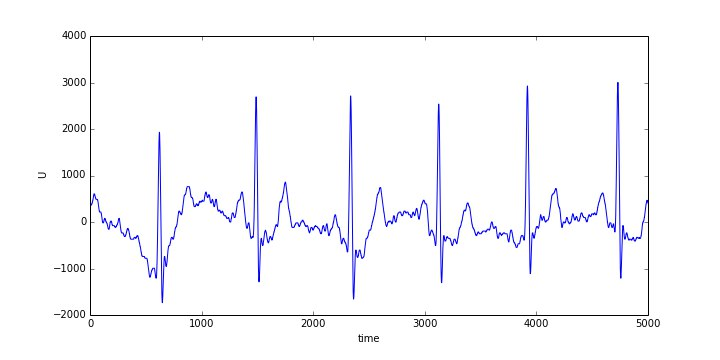
\includegraphics[scale=0.5]{real_ekg}
		\caption{ЭКГ}
		\label{ris:RR}
	\end{center}
\end{figure}
\subsubsection{Немного об устройстве сердца}

Сердце обладает рядом свойств.

\begin{itemize}
	\item Свойство автоматизма - это способность сердца вырабатывать электрические импульсы при отсутствии внешних раздражений.
	\item Свойство проводимости - это способность к проведению возбуждения волокон проводящей системы сердца и сократительного миокарда.
	\item Свойство возбудимости – это способность клеток проводящей системы сердца и сократительного миокарда возбуждаться под влиянием внешних электрических импульсов.
\end{itemize}

Возбуждение сердечной мышцы сопровождается возникновением изменяющейся разности потенциалов между наружной и внутренней поверхностью клеточной мембраны сердца.

При распространении по сердцу волны деполяризации наружная поверхность клетки приобретает отрицательный заряд, а во время реполяризации – положительный. Согласно концепции В. Эйнтховена, сердце в каждый момент сердечного цикла можно рассматривать как точечный единый диполь, который создает в окружающей его среде электрическое поле. Положительный полюс диполя (+) всегда обращен в сторону невозбужденного, а отрицательный полюс (–) – в сторону возбужденного участка сердца(рис. \ref{ris:dipol}).

\begin{figure}[h]
	\begin{center}
		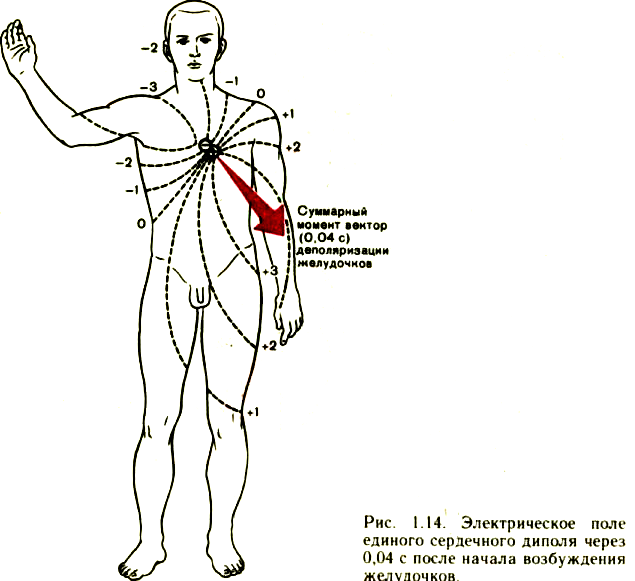
\includegraphics{heart-dipol}
		\caption{Поле сердечного диполя в отведениях}
		\label{ris:dipol}
	\end{center}
\end{figure}


Помещая положительный и отрицательный электроды в любые точки электрического поля, можно зарегистрировать разность потенциалов, существующую между этими точками в каждый момент деполяризации и реполяризации сердца. Конфигурация такой ЭКГ прежде всего будет зависеть от направления вектора диполя по отношению к электродам.

В настоящее время в клинической практике наиболее широко используют 12 отведений ЭКГ, запись которых является обязательной при каждом электрокардиографическом обследовании больного: 3 стандартных отведения, 3 усиленных однополюсных отведения от конечностей и 6 грудных отведений.

Стандартные отведения от конечностей регистрируют при следующем попарном подключении электродов:

\begin{itemize}
	\item I отведение – левая рука (+) и правая рука (–);
	\item II отведение – левая нога (+) и правая рука (–);
	\item III отведение – левая нога (+) и левая рука (–).
\end{itemize}

\subsection{RR}
Если рассматривать момент сокращения сердца более подробно \cite{polarization_heart} виден QRS-комплекс - изменения электрического потенциала, предшествующее сокращению сердца. За электрической активацией клеток (деполяризацией) следует механическое сокращение. Процесс сокращения сердечных мыщц состоит из следующих стадий (рис.\ref{ris:RR}).

\begin{itemize}
	\item деполяризация предсердий; зубец P
	\item передача импульса желудочкам; интервал PR
	\item деполяризация желудочков; зубец R
	\item реполярицазия желудочков; зубец T
	\item мнения исследователей относительно причин происхождения зубца V различны.
\end{itemize}

\begin{figure}[h]
	\begin{center}
		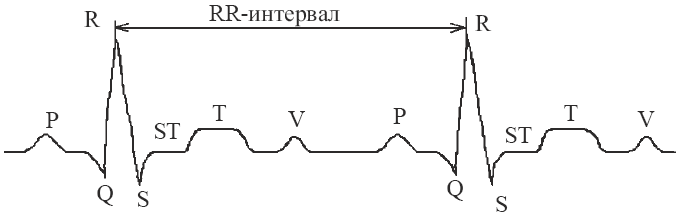
\includegraphics[scale = 0.5]{RR.png}
		\caption{ЭКГ}
		\label{ris:RR}
	\end{center}
\end{figure}

Для различных отведений вид QRS комплекс может отличаться. Вместо пика R может быть глубокий минимум. Минимумы Q, S могут отсутствовать. Приведенный на рисунке выше и на рис. примеры соответствуют первому отведению.

По длительности интервалов, глубине минимумов и высоте максимумов врачи предсказывают различные характеристики и болезни.

RR-интервалом называется промежуток времени между R пиками (последовательными ударами сердца). Нормально частотой серцебиения считается 60-100 ударов в минуту в состоянии покоя. Ниже приведены примеры RR-сигнала (последовательность RR-интервалов) (рис. \ref{real_RR}).

\begin{figure}[h]
	\begin{minipage}[h]{0.47\linewidth}
		\center{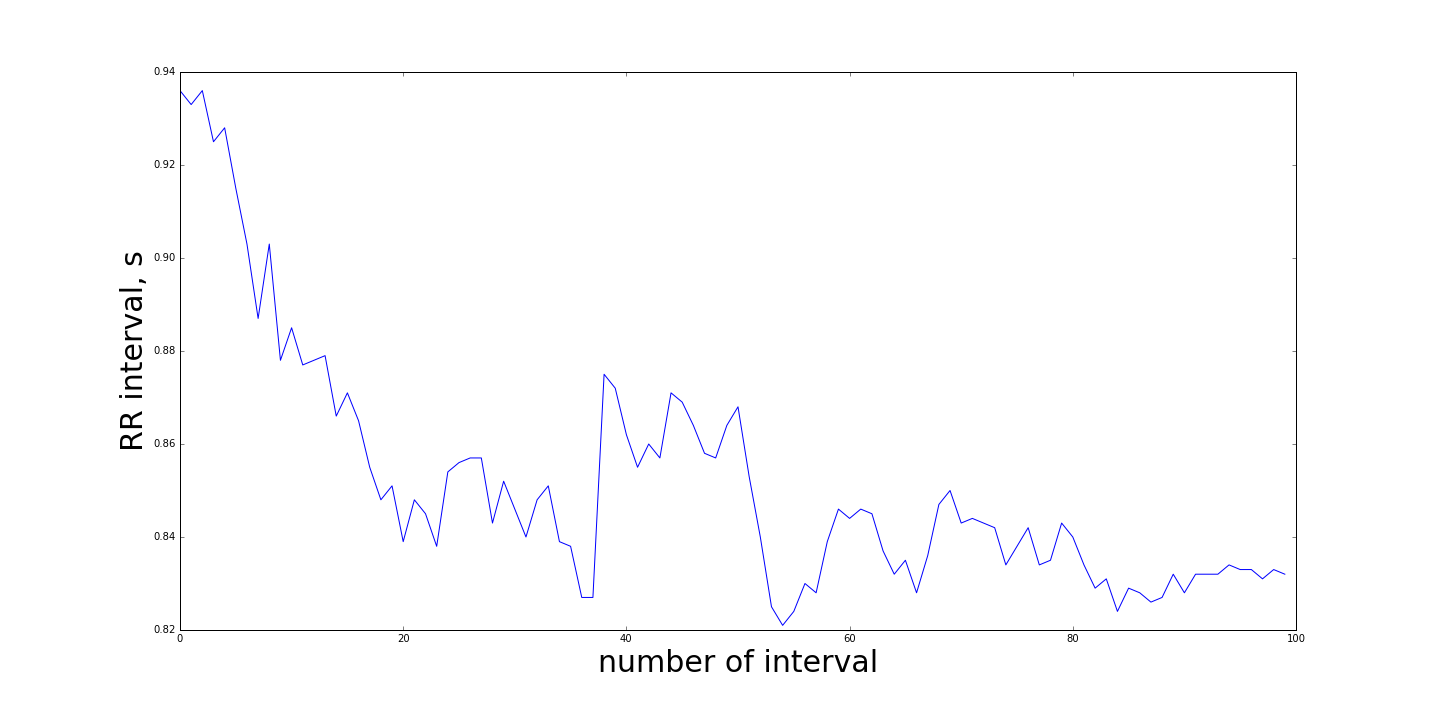
\includegraphics[width=1\linewidth]{rr_100}} a) \\
	\end{minipage}
	\hfill
	\begin{minipage}[h]{0.47\linewidth}
		\center{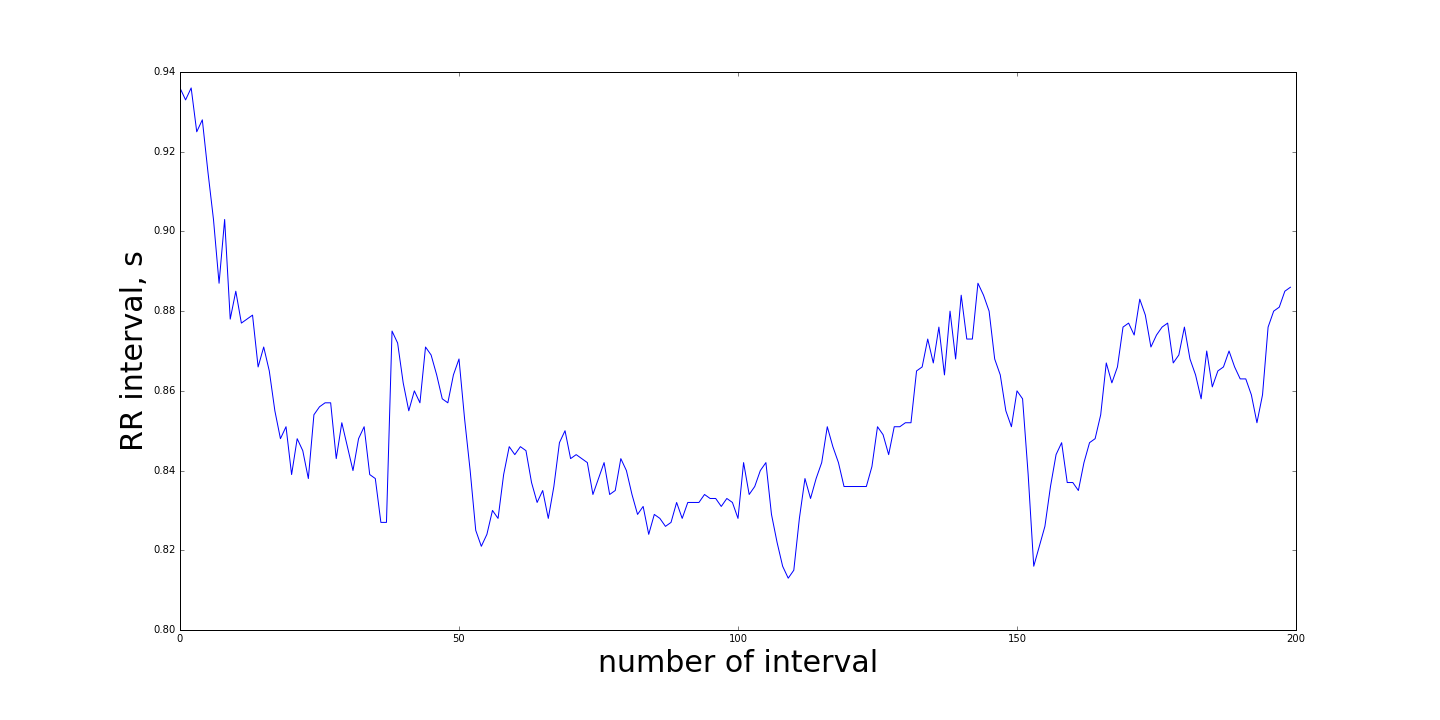
\includegraphics[width=1\linewidth]{rr_200}} \\b)
	\end{minipage}
	\vfill
	\begin{minipage}[h]{0.47\linewidth}
		\center{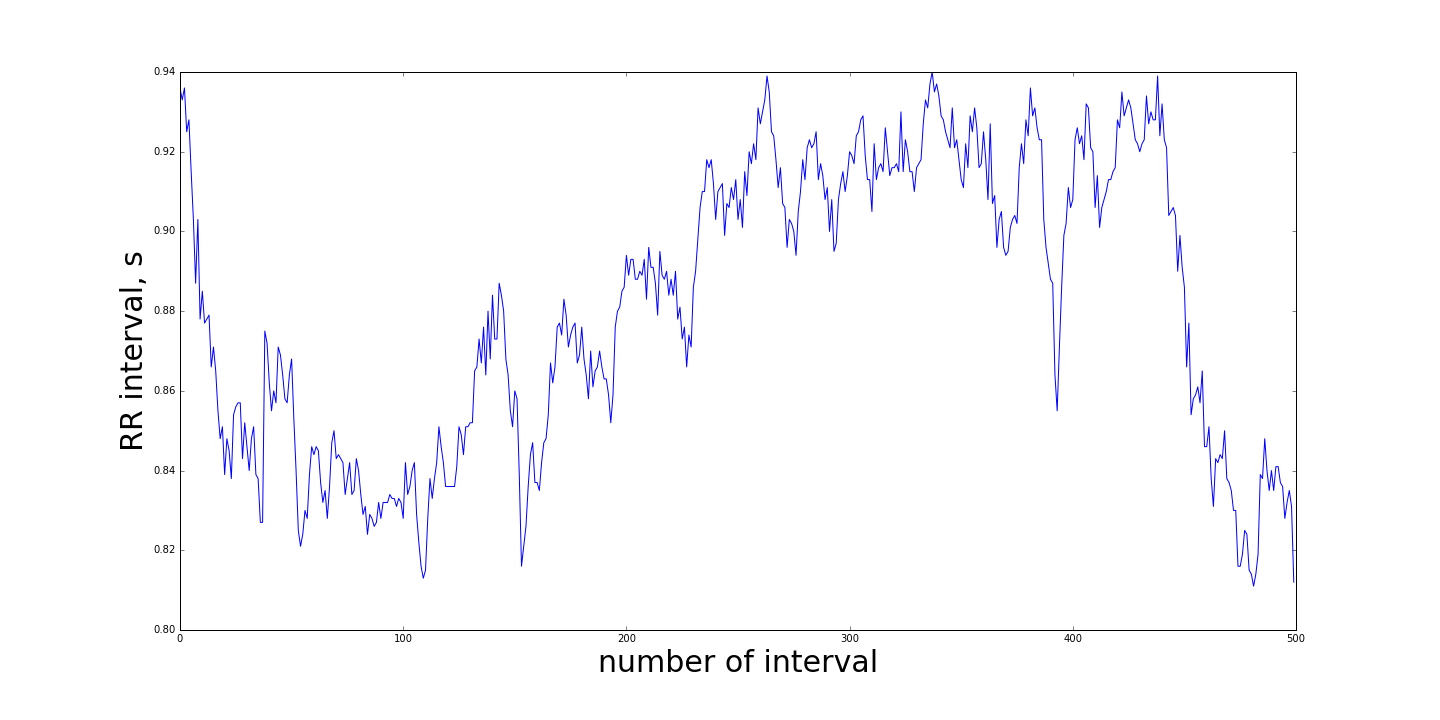
\includegraphics[width=1\linewidth]{rr_500}} c) \\
	\end{minipage}
	\hfill
	\begin{minipage}[h]{0.47\linewidth}
		\center{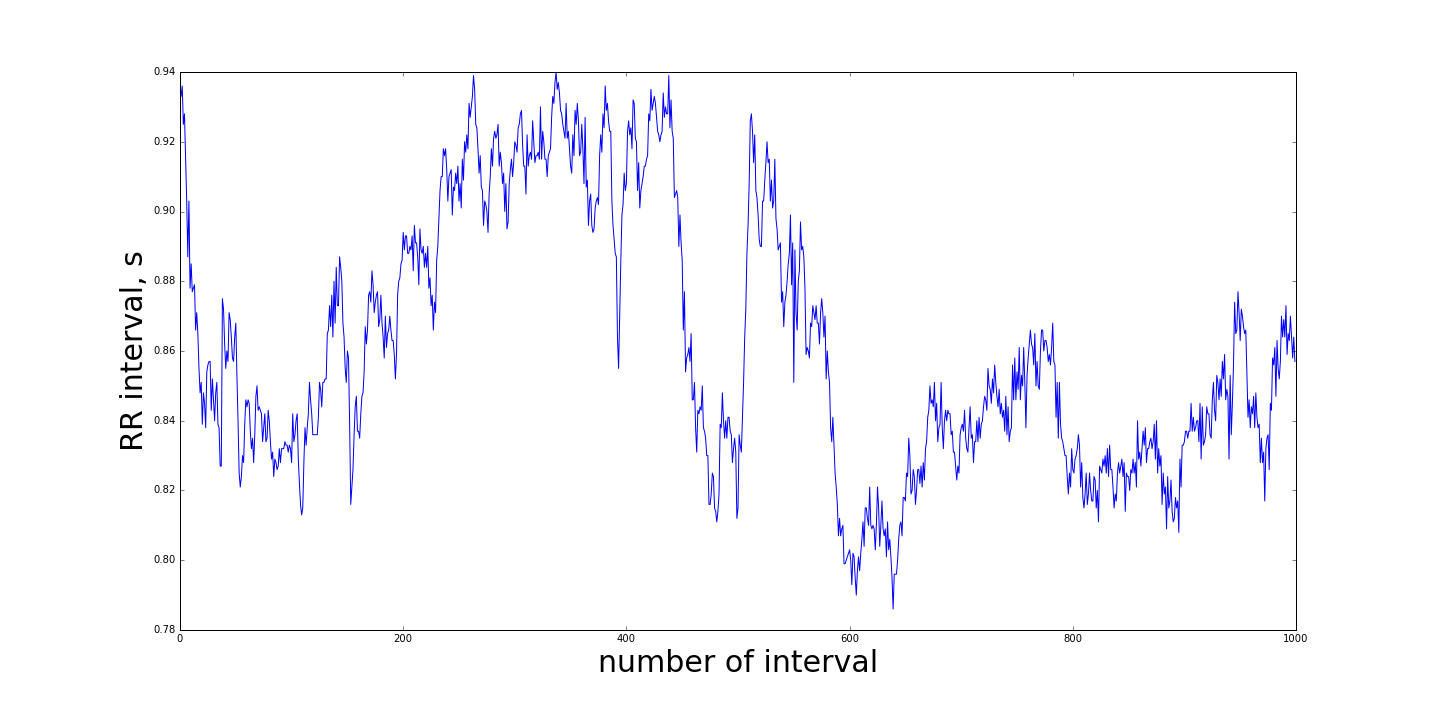
\includegraphics[width=1\linewidth]{rr_1000}} d) \\
	\end{minipage}
	\begin{minipage}[h]{0.47\linewidth}
		\center{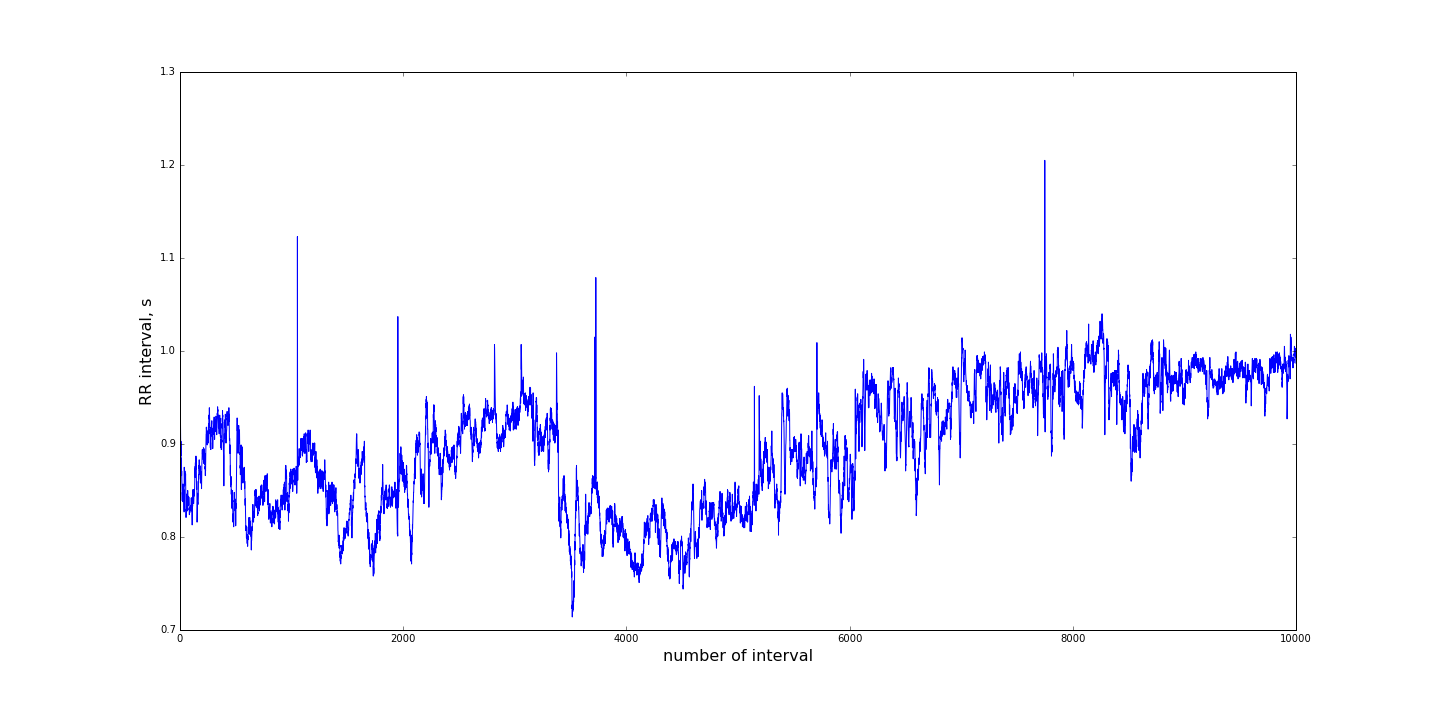
\includegraphics[width=1\linewidth]{rr_10000}} e) \\
	\end{minipage}
	\hfill
	\begin{minipage}[h]{0.47\linewidth}
		\center{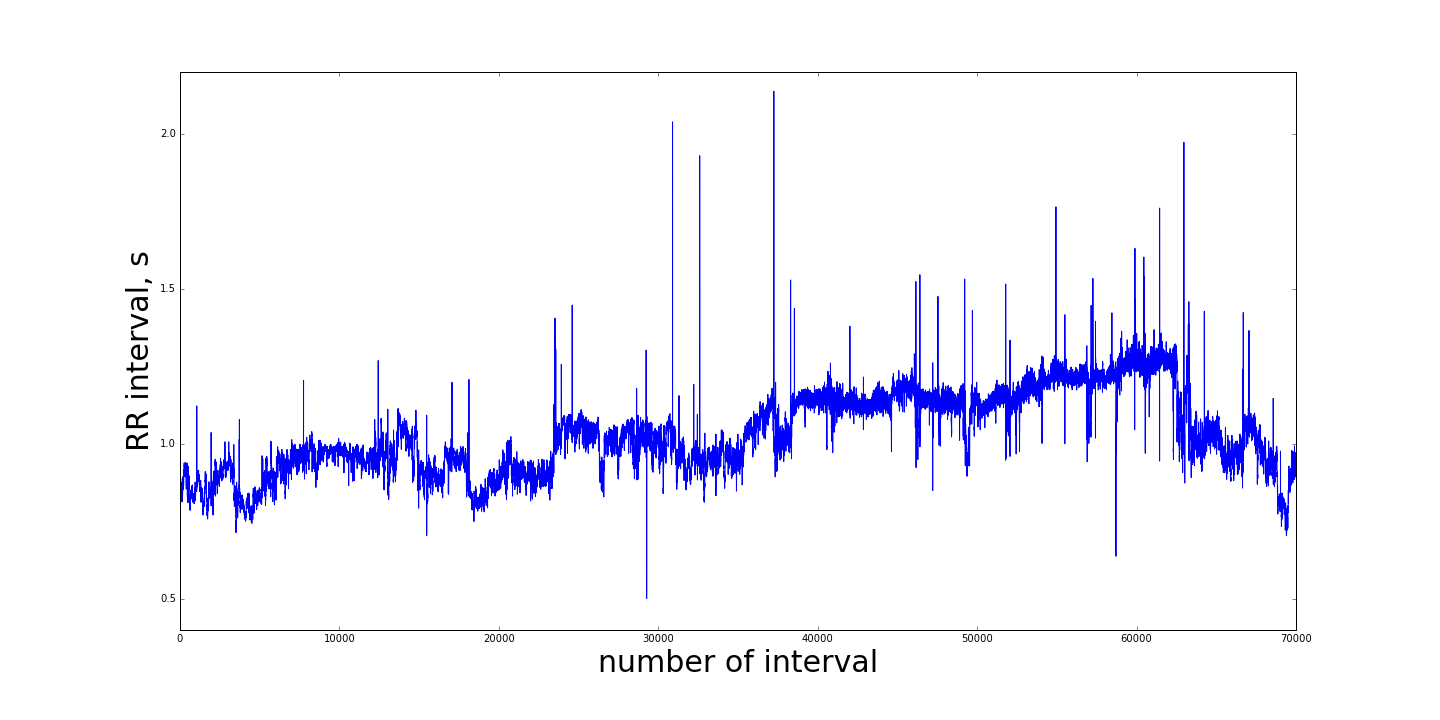
\includegraphics[width=1\linewidth]{rr_70000}} f) \\
	\end{minipage}
	\caption{RR-сигнал длительностью a)100 отсчетов $\sim$ 70с) b) 200 отсчетов
		c) 500 отсчетов d) 1000 отсчетов e)10000 отсчетов ($\sim $2 часа) f)70000 отсчетов.}
	\label{ris:reaal_RR}
\end{figure}


\subsection{Анализ RR сигнала}

Основные методы исследования HRV.

\begin{enumerate}
	\item Методы основанные на анализе интервалов между сердечными ударами NN типа. При данном анализе часто подсчитываются следующие характеристики \cite{pNN, metric_of_hrv}.
	\begin{enumerate}
		\item SDNN, стандартное отклонение интервалов NN от среднего, вычесленого почти всегда в течение 24 часов. SDNN обычно вычисляется для коротких интервалов, порядка 5 минут. SDNN отражает все циклические компоненты, ответственные за изменчивость в период записи, поэтому она представляет собой общую вариабельность.
		\item 	RMSSD ("среднеквадратичное последовательных различий»), квадратный корень из среднего значения квадратов последовательных разностей между соседними NN ударами.
		\item SDSD ("стандартное отклонение последовательных разностей"), стандартное отклонение последовательных разностей между соседними NNS.
		\item NN50, количество пар последовательных NN ударов, которые отличаются более чем 50 мс.
		\item pNN50, доля NN50 делится на общее количество NN ударов.
		\item 	NN20, количество пар последовательных NN ударов, которые отличаются более чем 20 мс.
		\item pNN20, доля NN20.
		\item EBS ("оценивается цикл дыхания"), диапазон (макс-мин) в скользящем окне заданной длительности. Окна можно перемещать без перекрытия или с перекрытием. ЕВС часто используют при сборе данных, где обратная связь ВСР в режиме реального времени является главной целью.
	\end{enumerate}
	\item Геометрические методы \cite{geometric_metric}
	\item Частотный анализ
	
	Строятся гистограммы частотных характеристик NN ударов
	
	\item Подсчет кореляций следующих NN ударов от предидущих \cite{autocorr_metric}
	\item Нелинейные методы \cite{non_linear_metric}
	
	\begin{enumerate}
		\item график Пуанкаре \cite{poinkare_plot}.
		\item фрактальные размерности \cite{fractal_dim}.
		\item флуктуационный анализ \cite{fluct_analis}
		\item энтропия \cite{entropy1, entropy2, entropy3}
		\item и др. \cite{other_analis1, other_analis2, other_analis3}
	\end{enumerate}	
\end{enumerate}

\section{Предсказание сна}
Сейчас 
\section{Рекуррентные нейронные сети}
Рекуррентная нейронная сеть – один из типов нейронных сетей \cite{neural_network}, в котором присутствует обратная связь. Другими словами в выход более позднего слоя сети поступает на вход более слоя, считающегося ранее.

Рекуррентные нейронные сети имеют ряд преимуществ перед обычными.
\begin{itemize}
	\item Разнообразные виды входных данных
	\item Способность строить неявные модели данных
	\item Устойчивость к выбросам
	\item 
\end{itemize}

Рекуррентные сети применяются в таких задачах как:
\begin{itemize}
	\item распознавание устной и письменной речи \cite{rnn_for_speech_recognition, rnn_for_text_recognition};
	\item машинный перевод \cite{rnn_for_translation};
	\item предсказания временных рядов \cite{rnn_for_prediction};
	\item И т.п.
\end{itemize}



Основной проблемой при использовании рекуррентных нейронных сетей является проблема исчезающего градиента (vanishing gradient problem \cite{vanishing_gradient_problem}). Если честно подсчитывать градиент на каждой итерации обучения он будет выражаться через произведение градиентов, подсчитанных на всех предыдущих итерация. Если градиенты были малы – наш градиент будет просто не заметен и обучение встанет надолго. 

Проблема исчезающего градиента была подробно рассмотрена Хочрайтером???(произношение) and Шмидхубера, которые разработали LTSM архитектуру \cite{create_lstm}, которая устойчива к данной проблеме. Данная архитектура оказалась проста в использовании и стала стандартным средством борьбы с исчезающим градиентом. Также были осуществлены попытки других способов решения данной проблемы:
\begin{itemize}
	\item обратное распостранение во времени (Backpropagation through time) \cite{Backpropagation}. Используется для обучения сетей Элмана.
	\item использование мощного secondorder алгоритмы оптимизации (Martens, 2010; Мартенс Sutskever, 2011)
	\item регуляризация весов в RNN, что гарантирует, что градиент не обращается в нуль (Pascanu др.,2012)
	\item отказ от всего обучения текущие веса (Jaeger, Haas, 2004; Jaeger, 2001), и очень
	осторожны инициализации параметров РНН (в Sutskever др.,2013).
\end{itemize}
	
Также была обнаружена проблема сильного возрастание градиента, но она легко решилась ограничение на модуль градиента.

\subsection{LSTM}

Данный слой успешно борется с проблеммай исчезающего градиента. Каждый нейрон в данном слое представняет собой "ячейку памяти" (рис. \ref{ris:ltsm}). Данные ячейки организованны для хранения информации и позволяют более качествеено обрабатывать длинные входные последовательности.

\begin{figure}[h]
\begin{center}
	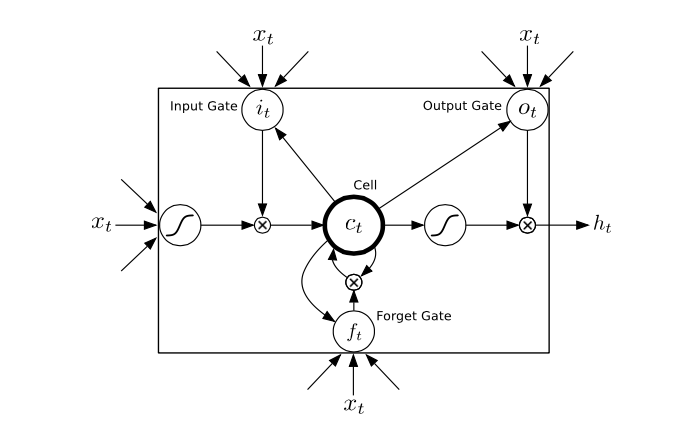
\includegraphics[scale=0.36]{ltsm.png}
	\caption{LSTM ячейка}
	\label{ris:ltsm}
\end{center}
\end{figure}


Пускай на вход LSTM ячейке памяти подается часть входной последовательности $x_t = (x_1, ..., x_N)$ и предыдущие выходной вектор признаков $h_{t-1} = (h_1, ..., h_M)$. Ячейка должна подсчитать вектор признаков $h_t$. Ячейка организованны следующим обрахом:


\begin{equation}
	i_i = \sigma(W_{xi}*x_t+W_{hi}*h_{t-1}+W_{ci}*c_{t-1}+b_i)
\end{equation}
\begin{equation}
	f_t = \sigma(W_{xf}*x_t+W_{hf}*h_{t-1}+W_{cf}*c_{t-1}+b_f)
\end{equation}
\begin{equation}
	c_t = f_t*c_{t-1}+i_t*\tanh(W_{xc}*x_{t-1}+W_{hc}*h_{t-1}+b_c)
\end{equation}
\begin{equation}
	o_t = \sigma(W_{xo}*x_t+W_{ho}*h_{t-1}+W_{co}*c_t+b_o)
\end{equation}
\begin{equation}
	h_t = o_t*\tanh(c_t)
\end{equation}

Здесь $\sigma = \frac{1}{1+e^{-x}} $ - сигмоида, логистическая функция, принимающая значения от 0 до 1. А i, f, o и c - вход ячейки, клетка памяти, выход ячейки и клетка активации, по содержимому которой решается, будет ли использоваться ектор из клетки памяти. Все вышеперечисленные вектора имеют размерность $h_t$.
\chapter{Основная часть}
\section{Имеющиеся данные}
В рамках программы SAHR были записаны ЭКГ (использовалось только первое отведение) 1800 москвичей преклонного возраста (55-91 год). Из них 46\% мужчин. Запись каждого ЭКГ производилась в течение суток. В это же время за человеком велось дополнительное наблюдение и было известно, в какой промежуток времени он спал, а в какой - бодрствовал. Также про каждого человека известна некоторая информация: состояние здоровья, вес, курит ли он и многое другое.
\section{Постановка задачи}

Цель работы - анализируя данные ЭКГ предсказать в какое время человек спал/бодроствовал, исследовать возможность предсказания болезней и самочувствия человека.Также в рамках обучени выделения признаков и их анализа были проведены исследования по идентификации человека.

\section{Актуальность задачи}
Электрокардиография - самый распространенный клинический инструмент, который измеряет электрическую деятельность сердца с поверхности тела. Сигнал ЭКГ, или проще вариабельности сердечного ритма содержит много интересной информации о человеке. Процесс получения информации об ЭКГ у людей стал простым !!!!!!!!(более технически простым) с изобретения новых технологий и приборов, таких как фитнесс-браслеты, специальные чехлы для телефонов, мониторы-холтеры и т. д. Также создание базы данных, собранных в дополнение к существующим (SAHR, AHA DB, ESC DB и т. д.). в настоящее время.

Процесс сна имеет важное значение для медицинской диагностики. Классическая полисомнография для мониторинга сна накладывает существенные ограничения на практике. В последние годы, носимых устройств для мониторинга здоровья становится все более популярными. Браслеты и смарт-часы позволяют пациенту быть подвижным, в то время как необходимые данные собираются в своей естественной среде. Однако, на сегодняшний день нет хороших научных доказательств, представленных публике, о том, что эти устройства могут оценить продолжительность сна с высокой точностью.

\section{Фильтрация ЭКГ сигнала и выделение RR-пиков}
\subsection{Фильтрация ЭКГ}
К экг сигналу применялся ряд фильтров: фильтры высоких и низких частот. 
тут будет картинки 4.
\subsection{Выделение RR-пиков}
Для определения RR-пиков использовалсz следующий алгоритм.

\begin{enumerate}
	\item На протяжении 200мс бралась точка максимального участока сигнала.
	\item Справа от него в течение 5 мс бралась минимальная точка и проверялось, что это локальний минимум.
	\item Разница высот между минимум и максимумом должна бть больше порогового значения.
	\item Проверялось, что слева от максимумfа в пределах 20 мс также можно найти точку, меньше чем максимум для заданного значения
\end{enumerate}

!!!иллюстрация алгоритма

\section{Работа с RR-сигналом}
\subsection{Отбор RR-пиков}
Для классификации промежутков времени на сон/бодрствование необходим весь временной ряд. Но для идентификации человека, для предсказания каких-либо характеристик достаточно только его части. Если брать для предсказания характеристик небольшие участки сигнала размер обучающей выборки увеличится в несколько раз, увеличится ее обобщающая способность.

То, что мы берем только участки сигнала позволяет нам отобрать участки с минимумом шума. На сигнал могут влиять случайные движения человека, непроизвольные сокращения мыщц. Может быть не очень хорошо закреплен электрод или же он может сдвинуться или отойти на время. в первом случае мы получаем лишние пики, во втором, наоборот, долгий промежуток без них. 

Было решено отбирать участки сигнала где все выделенные R-пики удовлетворяют следующим условиям:

\begin{itemize}
	\item RR интервалы больше 200 милисекунд
	\item RR интервалы меньше 2 секунд
	\item разница высот соседних пиков менее 20\%
	\item разница продолжительностей соседних RR интервалов менее 20\%
\end{itemize}
\subsection{Выделение признаков}
Признаки!много)
Большая часть подсчитываемых признаков по выделенным R пикам описана в обзоре литературы - они являются стандартными при работе в ЭКГ сигналом. Однако вдобавок к ним использовались еще добавочные признаки.
\begin{itemize}
	\item амплитуды пиком и минимумов в QRST-комплексе
	\item разница высот между пиками P, R, T
	\item отношения ввысот P, R, T
	\item средние значения на промежутках PQ, QR, QT
	\item длительнисть различных фаз в QRST-комплексе
	\item площадь под графиком на промеежутках PQ, QS, ST, begin-Q, S-final
\end{itemize}
В медицине утверждается [!! ссыдки], что врачи ориентируются на данные параметры при постановки диагноза.
\section{Проведенные экперименты}
В рамках данного исследовая проводились попытки решения следующих задач.
\subsection{Идентификация человека}
Люди делились на 3 выборки: тестовую, валидационную и обучающую. Экг каждого человека нарезались на отрезки. Состовлялись пары отрезков, для каждой пары устанавливалось из одного сигнала они взяты (1) или из разных (0). Далее пары отрезков подавались на вход сети :
 архитектуру? надо ли вообще. я об этом так себе знаю - это твое исследование было
Качество предсказания на тестовом датасете - 75\%. Количество элементов каждого класса во всех выборках было равным.
\subsection{Предсказание сна}
Предсказание сна - актуальная задача по следующим причинам.
В ходе данного исследования рассмативались следующие методы
\subsubsection{Линейный классификатор}
Если смотреть на RR-сигнал во время сна и бодроствования (две картинки сюда) можно заметить, что во время сна частота пульса уменьшается (достаточно очевидное предположение известное всем). Также на большей части ЭКГ уменьшается дисперсия сигнала во время сна.
Первым предложенным алгоритмом был следующий.
\begin{enumerate}
	\item для сигнала подсчитывались среднее значение и дисперсия
	\item маркируются все точки сигнала на три категории
	\begin{itemize}
		\item точки на половину дисперсии больше среднего значения
		\item точки на половину дисперсии меньше среднего значения
		\item все остальные точки (формулой бы?)
	\end{itemize}
	\item Далее мы ищем наиболее длинную последовательность точек из первой группы, не прерываемую более чем 5 точками из второй в лоюбом ее месте
\end{enumerate}
Количество точек было подобрано на обучающей выборке. (исправить - посмотреть, сколько точно)
Качество предсказания - 75\%.
Картинок сюда.
\subsubsection{Деревья}
Далее было принято решение увеличить количество признаков и кроме среднего и дисперсии посчитать стандартные приз
Далее было решено проверить следующее предположение: при работе с RR сигналом люди считают множество признаков - может быть не просто так. Давайте посчитаем их и на них что-нибудь обучим.
\subsection{Предсказание болезней}

\bibliography{biblio}
\addcontentsline{toc}{chapter}{Список литературы}
\end{document}